\documentclass[12pt]{article}
\usepackage{graphicx}

\topmargin 0.0cm
\oddsidemargin 0.2cm
\textwidth 16cm 
\textheight 21cm
\footskip 1.0cm

\title{Basic Expolaratory Data Analysis of Titanic Dataset} 


\author
{Nurislam Tursynbek\\
\\
\normalsize{Skolkovo Institute of Science and Technology}\\
\\
\normalsize{E-mail:  nurislam.tursynbek@skoltech.ru}
}

\date{}

\begin{document} 

\maketitle 

\newpage

\section{Introduction}

The sinking of the RMS Titanic is one of the most infamous shipwrecks in history.  On April 15, 1912, during her maiden voyage, the Titanic sank after colliding with an iceberg, killing 1502 out of 2224 passengers and crew. This sensational tragedy shocked the international community and led to better safety regulations for ships.

One of the reasons that the shipwreck led to such loss of life was that there were not enough lifeboats for the passengers and crew. Although there was some element of luck involved in surviving the sinking, some groups of people were more likely to survive than others, such as women, children, and the upper-class.

The data science platform Kaggle launched a competition several years ago, in which they ask to complete the analysis of what sorts of people were likely to survive. In particular, they ask to apply the tools of machine learning to predict which passengers survived the tragedy.

\section{Exploratory Data Analysis}

Here we do some basic exploratory analysis of the titanic dataset.

After looking a the structure of tables, let's visualise some plots.

Based on the domain knowledge, we assume that three most important features are 'Age', 'PClass', and 'Fare'. \\
It is logical: if you are younger, or if your class is better, or if your ticket is more expensive, then you are more likely to survive.

Let's draw scatter plots between these features.

\begin{figure}[ht!]
    \centering
    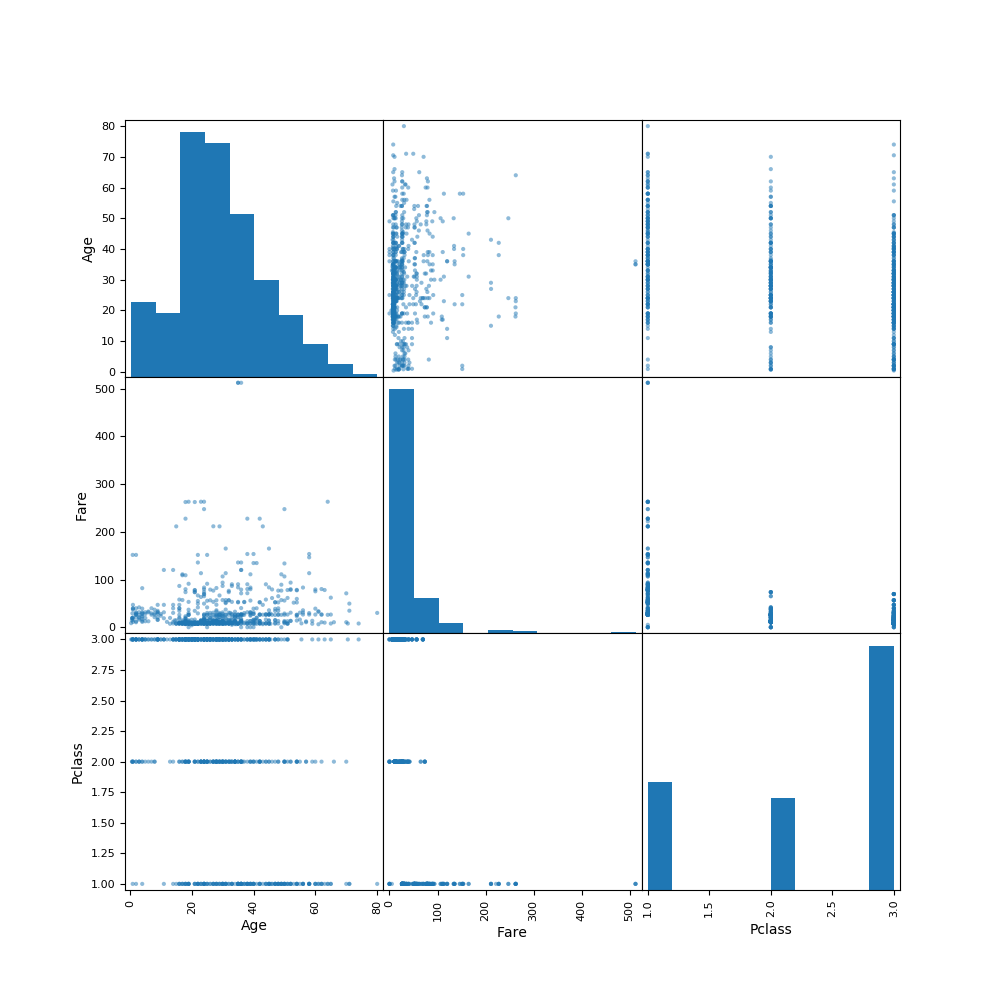
\includegraphics[width=0.4\textwidth]{figs/figure_1.png}
    \caption{Initial matrix of scatter plots of three most important features.}
\end{figure}

There are some passengers, whose ages are unknown, leading to some missing values in this column. Additionally there is one passenger, whose ticket's price is unknown, as well. To impute these, missing values, we first group passengers by Pclass and calculate medians of each group. Now we substitute missing values of each group with their corresponding medians.

Now let's draw scatter plots between these features.

\begin{figure}[ht!]
    \centering
    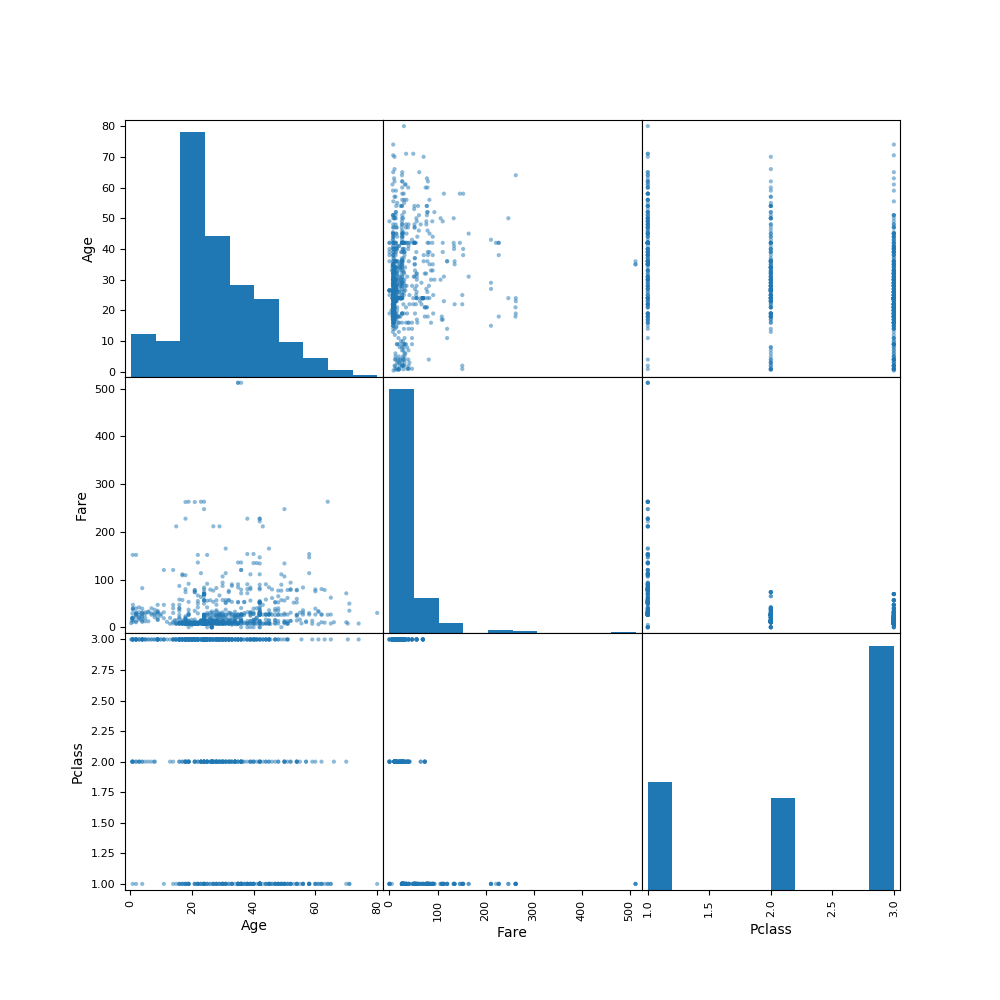
\includegraphics[width=0.4\textwidth]{figs/figure_2.png}
    \caption{Matrix of scatter plots of three most important features with imputed missing values.}
\end{figure}

\section{Regressions}

In this section we exploe the regression model to several pairs of features

Let's look at scatter plot of 'PClass' and 'Fare' separately.

\begin{figure}[ht!]
    \centering
    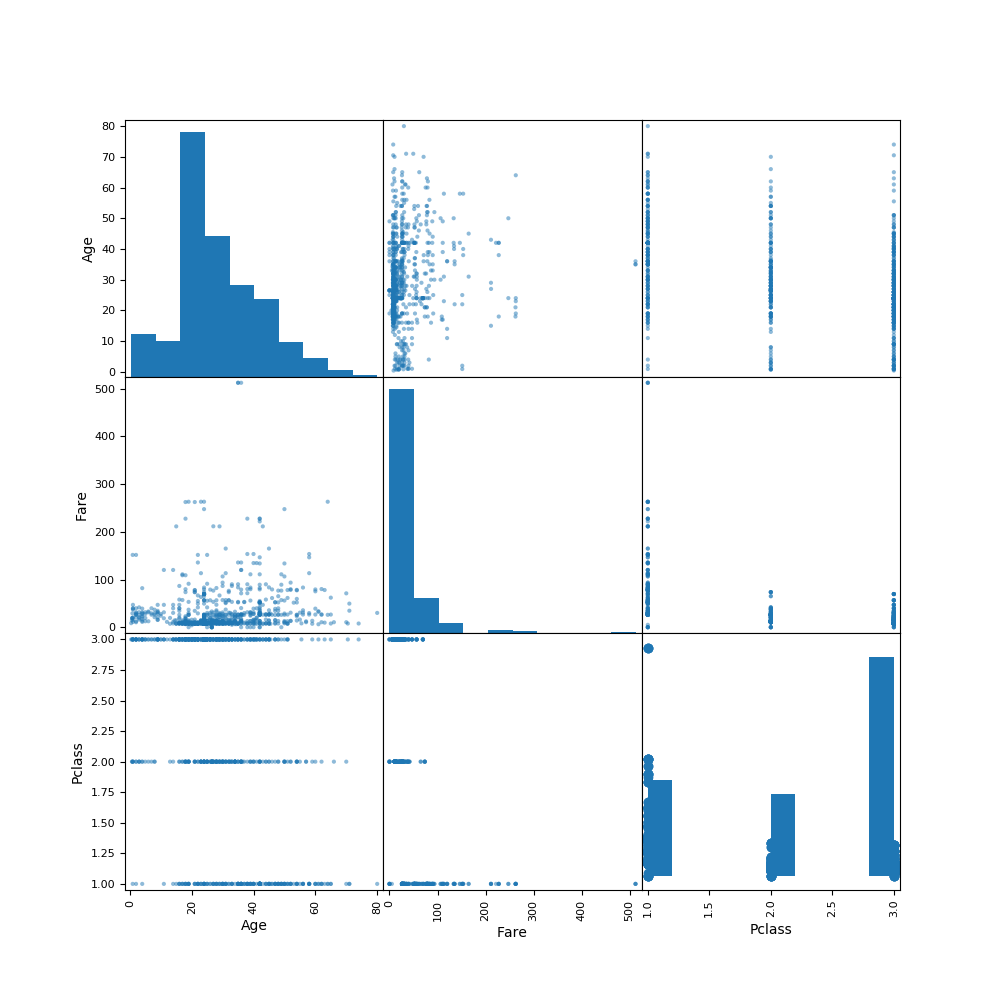
\includegraphics[width=0.4\textwidth]{figs/figure_3.png}
    \caption{Scatter plot of 'PClass' and 'Fare'.}
\end{figure}

We can calculate slope and intercept for least square regression line between this featues and plot it.

\begin{figure}[ht!]
    \centering
    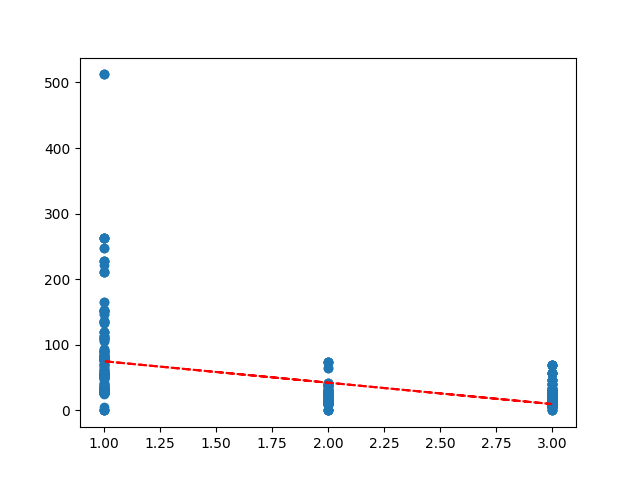
\includegraphics[width=0.4\textwidth]{figs/figure_4.png}
    \caption{Scatter plot of PClass' and 'Fare' with least square regression line.}
\end{figure}

We repeat the same plots for 'Age' and 'PClass' case.

\begin{figure}[ht!]
    \centering
    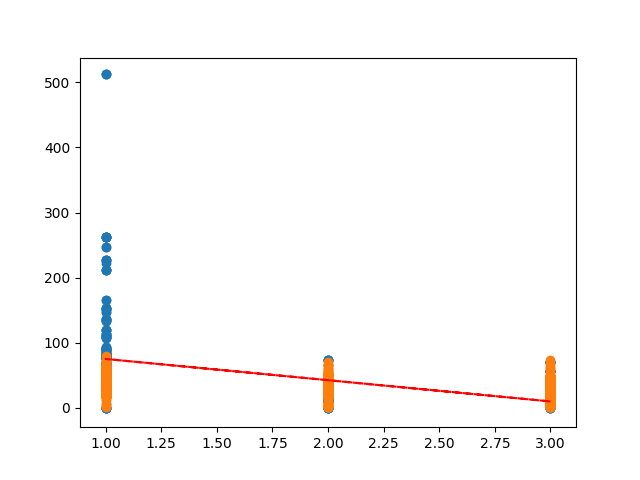
\includegraphics[width=0.4\textwidth]{figs/figure_5.png}
    \caption{Scatter plot of 'PClass' and 'Age'.}
\end{figure}
 
\begin{figure}[ht!]
    \centering
    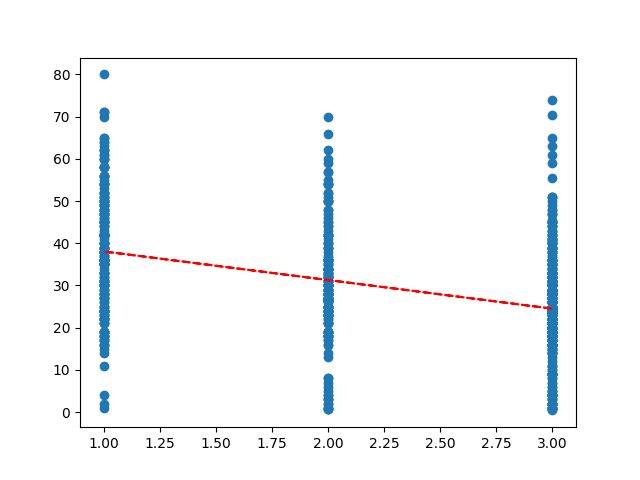
\includegraphics[width=0.4\textwidth]{figs/figure_6.png}
    \caption{Scatter plot of 'PClass' and 'Age' with least square regression line.}
\end{figure}

We repeat the same plots for 'Age' and 'Fare' case.

\begin{figure}[ht!]
    \centering
    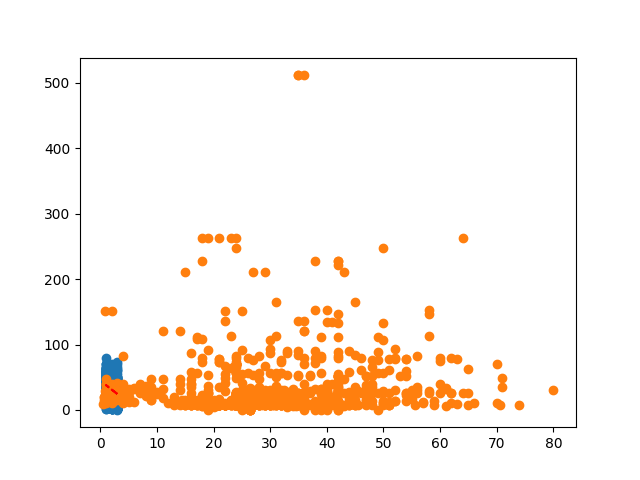
\includegraphics[width=0.4\textwidth]{figs/figure_7.png}
    \caption{Scatter plot of 'Age' and 'Fare'.}
\end{figure}

\begin{figure}[ht!]
    \centering
    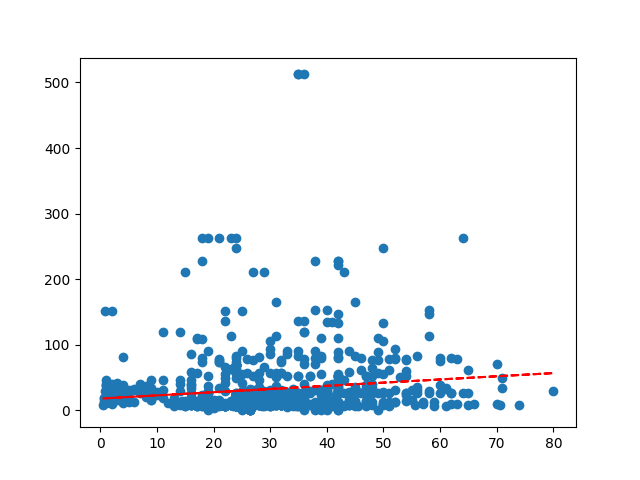
\includegraphics[width=0.4\textwidth]{figs/figure_8.png}
    \caption{Scatter plot of 'Age' and 'Fare' with least square regression line.}
\end{figure}

\end{document}
